\section{Datos}
\label{sec:data}

Esta secci\'{o}n describe los seis conjuntos de microdatos armonizados por pa\'{i}s y documenta el procedimiento de armonizaci\'{o}n ocupacional sobre el que descansa la estrategia de identificaci\'{o}n de la \cref{sec:method}. La unidad de armonizaci\'{o}n es la ocupaci\'{o}n CIUO-08 a cuatro d\'{i}gitos, el clasificador internacional de la OIT que sirve como puente com\'{u}n entre los clasificadores nacionales heterog\'{e}neos de la regi\'{o}n y las medidas de exposici\'{o}n a LLM construidas sobre O*NET y SOC. Comienzo con el caso del Per\'{u}, donde el desaf\'{i}o de armonizaci\'{o}n es m\'{a}s severo y donde su soluci\'{o}n marca el est\'{a}ndar para los pa\'{i}ses restantes.

\subsection{Per\'{u}: un cambio de clasificador que coincide con el shock}
\label{subsec:data_peru}

La fuente \emph{principal} para el Per\'{u} es la Encuesta Permanente de Empleo Nacional (EPEN) del Instituto Nacional de Estad\'{i}stica e Inform\'{a}tica (INEI), m\'{o}dulo que cubre Lima Metropolitana con frecuencia mensual y que agrego a frecuencia trimestral para alinearlo con la ventana muestral 2021T1--2025T4 del art\'{i}culo. La EPEN sustituy\'{o} en su funci\'{o}n trimestral al m\'{o}dulo de empleo de la Encuesta Nacional de Hogares (ENAHO) tras el redise\~{n}o muestral de 2023 del INEI. Toda la estrategia de identificaci\'{o}n descansa en la EPEN; la ENAHO se utiliza \'{u}nicamente como fuente de validaci\'{o}n anual en la secci\'{o}n de robustez, donde su cobertura nacional permite contrastar el resultado limeño con un agregado representativo del pa\'{i}s. La cobertura geogr\'{a}fica restringida de la EPEN se reconoce expl\'{i}citamente: el ACRT estimado $\hat\tau^{\text{Per\'{u}}}$ debe leerse como espec\'{i}fico de Lima Metropolitana y no como una afirmaci\'{o}n nacionalmente representativa.

El reto t\'{e}cnico central de la EPEN es que cambia de clasificador ocupacional a mitad de la ventana muestral, y el cambio coincide casi exactamente con la fecha de tratamiento. De 2021T1 a 2022T3, la EPEN codifica la ocupaci\'{o}n usando el C\'{o}digo de Ocupaciones de 1995 (CO-1995) a tres d\'{i}gitos: 319 c\'{o}digos aparecen al menos una vez en el per\'{i}odo, de un total de 370 c\'{o}digos definidos en el clasificador oficial del INEI. A partir de 2022T4, la EPEN migra al C\'{o}digo Nacional de Ocupaciones de 2015 (CNO-2015) a cuatro d\'{i}gitos, con 473 c\'{o}digos definidos en el clasificador. El corte cae en el mismo trimestre que la fecha de tratamiento $t^{\ast} = 2022\text{T4}$, lo que crea un riesgo de identificaci\'{o}n inmediato: cualquier salto mec\'{a}nico introducido por el cambio de granularidad se confundir\'{i}a con el efecto causal del lanzamiento de ChatGPT. Adem\'{a}s, el mapeo de CO-1995 a tres d\'{i}gitos hacia CNO-2015 a cuatro d\'{i}gitos es \emph{one-to-many}: un c\'{o}digo CO-1995 t\'{i}picamente se desagrega en varios c\'{o}digos CNO-2015. Mantener el CNO-2015 a cuatro d\'{i}gitos como unidad de an\'{a}lisis exigir\'{i}a, por tanto, imputar la asignaci\'{o}n de los trabajadores del per\'{i}odo previo a c\'{o}digos m\'{a}s finos sobre la base de informaci\'{o}n que la propia EPEN no recoge en esos trimestres. Mantener el CO-1995 a tres d\'{i}gitos como unidad sacrificar\'{i}a la mitad de la variaci\'{o}n ocupacional en exposici\'{o}n a LLM dentro de cada uno de esos c\'{o}digos, justamente la variaci\'{o}n que la literatura sobre exposici\'{o}n a IA y a LLM \citep{Felten2023_ai_exposure, Webb2020_ai_exposure, Eloundou2023_gpt_exposure} explota como ex\'{o}gena.

\subsubsection*{Armonizaci\'{o}n a CIUO-08 y validaci\'{o}n de la imputaci\'{o}n}

La estrategia adoptada lleva ambos per\'{i}odos a CIUO-08 a cuatro d\'{i}gitos, el clasificador internacional de la OIT, usando las cuatro tablas oficiales de correspondencia publicadas por el INEI.\footnote{Tablas de correspondencia descargadas del portal oficial del INEI: \url{https://www.inei.gob.pe/media/Tablas_de_correspondencia_CNO_CIUO_CO.xlsx}. La copia exacta utilizada se deposita en el paquete de replicaci\'{o}n.} La elecci\'{o}n de CIUO-08 como clasificador maestro tiene tres motivos: las medidas de exposici\'{o}n a IA est\'{a}n definidas a nivel SOC con crosswalk oficial a CIUO-08 \citep{Felten2023_ai_exposure, Webb2020_ai_exposure, Eloundou2023_gpt_exposure}, los otros cinco pa\'{i}ses del art\'{i}culo se armonizan tambi\'{e}n a ese clasificador, y el INEI dise\~{n}\'{o} el CNO-2015 alineado con CIUO-08 (90.1 por ciento de los c\'{o}digos CNO-2015 mapean a un \'{u}nico c\'{o}digo CIUO-08). En el per\'{i}odo post (CNO-2015), el mapeo a CIUO-08 v\'{i}a el Anexo~3 del INEI es directo. En el per\'{i}odo pre (CO-1995), encadeno los Anexos 2 y 3 con un esquema de pesos posteriores emp\'{i}ricos estimados sobre el propio post, condicionados en sexo, educaci\'{o}n, sector ISIC y dominio del trabajador. El procedimiento completo (ecuaci\'{o}n de los pesos posteriores, supuesto identificador del crosswalk y resultados detallados de las tres pruebas de validaci\'{o}n) se reporta en el \cref{app:peru_imputation}.

Las pruebas de validaci\'{o}n que pueden ejecutarse antes del DiD pasan los criterios pre-registrados en el plan de an\'{a}lisis. La diferencia m\'{a}xima entre shares de empleo CIUO en 2022T3 (\'{u}ltimo trimestre del pre, asignado v\'{i}a pesos posteriores) y 2022T4 (primer trimestre del post, asignado v\'{i}a el Anexo~3) es 2.05 puntos porcentuales, por debajo del umbral de cinco puntos porcentuales pre-registrado como evidencia de armonizaci\'{o}n problem\'{a}tica; la mediana es 0.04. La divergencia de Kullback-Leibler agregada de los pesos posteriores entre subper\'{i}odos del post es 0.046 nats en el peor caso (entre 2023 y 2025), bajo el umbral pre-registrado de 0.05 nats. Las pruebas que requieren el DiD estimado (tendencias previas a nivel armonizado y donut DiD que excluye los dos trimestres que cubren el corte) se reportan junto con los resultados en la \cref{sec:results} y en la secci\'{o}n de robustez.

\subsubsection*{Escalera de robustez sobre el clasificador}

La especificaci\'{o}n peruana se reporta a lo largo de cinco columnas para acotar la sensibilidad del resultado a las decisiones de armonizaci\'{o}n.

\begin{table}[H]
\centering
\small
\begin{threeparttable}
\caption{Escalera de robustez del clasificador para Per\'{u}}
\label{tab:peru_classifier_ladder}
\begin{tabular}{lll}
\toprule
Especificaci\'{o}n & Granularidad & Imputaci\'{o}n del per\'{i}odo pre \\
\midrule
\textbf{Principal} & CIUO-08 4d & Pesos posteriores condicionales en $X$ \\
Robustez 1 & CIUO-08 4d & Pesos uniformes \\
Robustez 2 & CO-1995 3d (Anexo 1 al post) & Ninguna (\emph{many-to-one}, sin imputaci\'{o}n) \\
Robustez 3 & CIUO-08 4d & Pesos post., donut excluye 2022T3--2022T4 \\
Robustez 4 & CIUO-08 4d & Solo per\'{i}odo post (DiD pre/post impl\'{i}cito) \\
\bottomrule
\end{tabular}
\begin{tablenotes}[flushleft]
\footnotesize
\item \emph{Notas:} La especificaci\'{o}n principal usa pesos posteriores estimados sobre 2022T4--2025T4 v\'{i}a la \cref{eq:posterior_weights}. Robustez 1 sustituye los pesos por una asignaci\'{o}n uniforme entre c\'{o}digos hijos. Robustez 2 colapsa el post a CO-1995 a tres d\'{i}gitos v\'{i}a el Anexo~1 (mec\'{a}nicamente exacto, sin supuestos de imputaci\'{o}n) a costa de menor granularidad. Robustez 3 elimina los trimestres 2022T3 y 2022T4 del estimador. Robustez 4 elimina por completo el per\'{i}odo pre y estima un DiD pre/post impl\'{i}cito sobre el post (placebo cruzado a nivel ocupacional sirve como prueba previa). Convergencia entre las cinco columnas se interpreta como evidencia de que el resultado peruano no es artefacto del cambio de clasificador.
\end{tablenotes}
\end{threeparttable}
\end{table}

\subsection{Los otros cinco pa\'{i}ses}
\label{subsec:data_others}

Los cinco pa\'{i}ses restantes presentan retos de armonizaci\'{o}n menos severos que el peruano y se documentan brevemente. Costa Rica (Encuesta Continua de Empleo, ECE), Colombia (Gran Encuesta Integrada de Hogares, GEIH), Ecuador (Encuesta Nacional de Empleo, Desempleo y Subempleo, ENEMDU) y Uruguay (Encuesta Continua de Hogares, ECH) publican microdatos codificados directamente en CIUO-08 a cuatro d\'{i}gitos, sin requerir crosswalks. M\'{e}xico (Encuesta Nacional de Ocupaci\'{o}n y Empleo, ENOE) publica en SINCO (Sistema Nacional de Clasificaci\'{o}n de Ocupaciones), que mapeo a CIUO-08 a cuatro d\'{i}gitos usando el crosswalk oficial SINCO-CIUO publicado por el INEGI. La tasa de coincidencia SINCO-CIUO al nivel de cuatro d\'{i}gitos es del 97.4 por ciento sobre los c\'{o}digos con empleo positivo en la ENOE 2021--2025; los c\'{o}digos sin coincidencia se asignan al nivel de tres d\'{i}gitos como en el procedimiento general descrito en la \cref{subsec:method_treatment}.

% TODO: tabla resumen por pa\'{i}s con (encuesta, frecuencia nativa, clasificador nativo, crosswalk usado, tasa de coincidencia 4d, n\'{u}mero de c\'{o}digos activos, tama\~{n}o muestral promedio por trimestre o a\~{n}o).

% TODO: subsecci\'{o}n con definici\'{o}n de variables de resultado armonizadas (empleo, horas, log salario por hora) y procedimiento de winsorizaci\'{o}n.

% TODO: subsecci\'{o}n con definici\'{o}n armonizada de formalidad por pa\'{i}s, siguiendo el protocolo descrito en la \cref{subsec:method_heterogeneity}, con especial cuidado en pa\'{i}ses donde la formalidad se identifica por contribuci\'{o}n a la seguridad social (Colombia, Costa Rica) frente a pa\'{i}ses donde se identifica por contrato escrito (M\'{e}xico) o por una combinaci\'{o}n (Ecuador, Per\'{u}, Uruguay).

\subsection{Estad\'{i}sticas descriptivas y primeros hallazgos}
\label{subsec:data_descriptives}

La fuerza laboral de Lima Metropolitana en 2021 se caracteriza por una edad media de 37.7 a\~{n}os (DE 12.5), una participaci\'{o}n femenina de 44.9 por ciento, una share con educaci\'{o}n terciaria o no universitaria postsecundaria de 36.3 por ciento, una tasa de formalidad de 36.7 por ciento bajo la definici\'{o}n basada en \texttt{seguro1}, una jornada media de 43.4 horas semanales y un logaritmo del salario por hora promedio de 1.88. La \cref{tab:peru_yearly} reporta la evoluci\'{o}n de los principales agregados a lo largo de la ventana 2021--2025.

\begin{table}[H]
\centering
\small
\begin{threeparttable}
\caption{Agregados anuales del panel armonizado, Lima Metropolitana}
\label{tab:peru_yearly}
\begin{tabular}{c c c c c c c}
\toprule
A\~{n}o & Trabajadores & Empleo expandido & \% formal & Horas medias & log salario hora & $\beta$ medio \\
\midrule
2021 & 28{,}814 & 4{,}267{,}694 & 37.7 & 43.4 & 1.91 & 0.280 \\
2022 & 31{,}241 & 4{,}618{,}022 & 39.6 & 44.5 & 1.97 & 0.282 \\
2023 & 24{,}376 & 4{,}915{,}388 & 42.2 & 45.1 & 2.06 & 0.286 \\
2024 & 22{,}449 & 5{,}134{,}375 & 41.7 & 44.9 & 2.12 & 0.289 \\
2025 & 21{,}777 & 5{,}268{,}328 & 43.2 & 45.7 & 2.18 & 0.290 \\
\bottomrule
\end{tabular}
\begin{tablenotes}[flushleft]
\footnotesize
\item \emph{Notas:} Trabajadores reporta el conteo \'{u}nico de identificadores hogar-persona-trimestre por a\~{n}o. Empleo expandido es el promedio anual de la suma trimestral del factor de expansi\'{o}n. Las columnas de outcomes son medias ponderadas por empleo expandido. La definici\'{o}n de formalidad es \texttt{seguro1} $\in \{1, 3\}$ (afiliaci\'{o}n a ESSALUD o esquema combinado). El $\beta$ medio es la exposici\'{o}n complementaria de \citet{Eloundou2023_gpt_exposure} ponderada por la composici\'{o}n ocupacional del a\~{n}o.
\end{tablenotes}
\end{threeparttable}
\end{table}

La distribuci\'{o}n de la exposici\'{o}n $\beta$ ponderada por empleo en 2021 tiene media 0.280 y desviaci\'{o}n est\'{a}ndar 0.178, con percentiles $p_{10} = 0.034$, $p_{25} = 0.146$, $p_{50} = 0.255$, $p_{75} = 0.400$ y $p_{90} = 0.503$. Aproximadamente el 25.6 por ciento de los trabajadores de Lima en 2021 ocupan posiciones con $\beta = 0$, mayoritariamente trabajos manuales no rutinarios y operativos. La \cref{fig:peru_beta_dist} reporta la densidad de $\beta$ separando los segmentos formal e informal de l\'{i}nea base.

\begin{figure}[H]
\centering
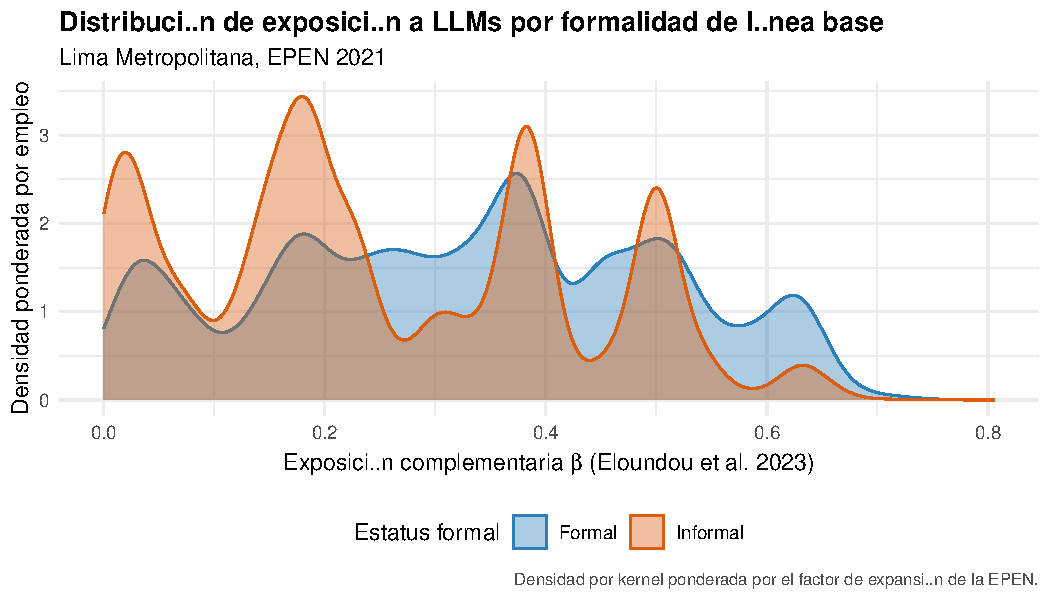
\includegraphics[width=0.85\textwidth]{figures/peru/fig_beta_distribution.pdf}
\caption{\textit{Densidad de la exposici\'{o}n complementaria $\beta$ por estatus de formalidad, Lima Metropolitana 2021.} La curva con relleno gris oscuro corresponde a trabajadores formales (\texttt{seguro1} $\in \{1, 3\}$) y la curva punteada con relleno gris claro a trabajadores informales. Las densidades est\'{a}n ponderadas por el factor de expansi\'{o}n trimestral de la EPEN.}
\label{fig:peru_beta_dist}
\end{figure}

Las dos colas de la distribuci\'{o}n est\'{a}n descritas en el \cref{app:peru_extremes}. La cola de alta exposici\'{o}n agrupa ocupaciones cognitivas profesionales (relaciones p\'{u}blicas, traductores, programadores de aplicaciones, escritores, matem\'{a}ticos, oficiales de cr\'{e}dito), todas concentradas en oficios cognitivos no rutinarios donde la sustituci\'{o}n parcial mediante software construido sobre LLM es plausible. La cola de baja exposici\'{o}n agrupa ocupaciones manuales y operativas (limpiadores de veh\'{i}culos, obreros de construcci\'{o}n, pintores, ayudantes de cocina), donde el contenido de tarea es f\'{i}sico y la complementariedad con LLM es estructuralmente baja.

La \cref{tab:peru_beta_formal} cruza los cuartiles de exposici\'{o}n con la share de formalidad para 2021 y entrega el hallazgo descriptivo m\'{a}s relevante para la estrategia de identificaci\'{o}n del art\'{i}culo: la formalidad se duplica entre el cuartil m\'{a}s expuesto y el menos expuesto. Las ocupaciones de alta exposici\'{o}n son sistem\'{a}ticamente m\'{a}s formales en la l\'{i}nea base.

\begin{table}[H]
\centering
\small
\begin{threeparttable}
\caption{Formalidad por cuartil de exposici\'{o}n $\beta$, Lima Metropolitana 2021}
\label{tab:peru_beta_formal}
\begin{tabular}{l c c c}
\toprule
Cuartil de $\beta$ & $\beta$ mediana & \% formal & Share del empleo (\%) \\
\midrule
Q1 (m\'{a}s baja)  & 0.034 & 25.8 & 25.1 \\
Q2                 & 0.188 & 30.0 & 25.4 \\
Q3                 & 0.375 & 41.0 & 25.6 \\
Q4 (m\'{a}s alta)  & 0.500 & 50.6 & 23.9 \\
\bottomrule
\end{tabular}
\begin{tablenotes}[flushleft]
\footnotesize
\item \emph{Notas:} Cuartiles de $\beta$ ponderados por empleo expandido en la EPEN 2021. La columna ``\% formal'' reporta la share de trabajadores con \texttt{seguro1} $\in \{1, 3\}$ dentro de cada cuartil.
\end{tablenotes}
\end{threeparttable}
\end{table}

\paragraph{Primeras conclusiones descriptivas.} Del cuadro descriptivo emergen tres patrones que orientan la estrategia de identificaci\'{o}n.

La exposici\'{o}n a LLMs en Lima Metropolitana resulta heterog\'{e}nea pero no extrema. La mediana ponderada por empleo es 0.255. La cola superior llega a 0.806 en relaciones p\'{u}blicas. La cola inferior concentra a un cuarto de los trabajadores en posiciones con $\beta = 0$. Esa distribuci\'{o}n no se concentra en un valor central. Ofrece, por lo mismo, variaci\'{o}n suficiente para estimar la dosis-respuesta a lo largo de la l\'{i}nea continua de tratamiento.

Un segundo patr\'{o}n, m\'{a}s relevante para la identificaci\'{o}n, es que los segmentos formal e informal de l\'{i}nea base ocupan posiciones distintas en la distribuci\'{o}n de exposici\'{o}n. La probabilidad de formalidad en una ocupaci\'{o}n del cuartil m\'{a}s expuesto (50.6 por ciento) duplica la del cuartil menos expuesto (25.8 por ciento). Esta correlaci\'{o}n est\'{a} predeterminada respecto al lanzamiento de ChatGPT, y por lo tanto refleja una caracter\'{i}stica estructural del mercado laboral peruano y no una respuesta al shock. Esa misma correlaci\'{o}n explica por qu\'{e} la heterogeneidad por formalidad es probablemente la dimensi\'{o}n con mayor magnitud emp\'{i}rica: la adopci\'{o}n de software complementario con LLM se concentra en firmas formales con capacidad de inversi\'{o}n y soporte tecnol\'{o}gico. Los efectos fijos de ocupaci\'{o}n absorben la correlaci\'{o}n de l\'{i}nea base y dejan la variaci\'{o}n intra-ocupaci\'{o}n como fuente del par\'{a}metro.

Un tercer hallazgo es que la propia composici\'{o}n ocupacional se est\'{a} desplazando lentamente hacia ocupaciones m\'{a}s expuestas durante el per\'{i}odo muestral. El $\beta$ medio ponderado por empleo sube de 0.280 en 2021 a 0.290 en 2025. El cambio es modesto. Aun as\'{i}, sugiere reasignaci\'{o}n a favor de ocupaciones expuestas, un margen extensivo cuya causalidad no es identificable directamente con esta especificaci\'{o}n pero que motiva el an\'{a}lisis de empleo expandido por celda en la \cref{sec:results}.

\paragraph{Construcci\'{o}n de celdas para el DiD.} Los microdatos armonizados se colapsan a la celda (CIUO-08 4d, trimestre) ponderando por empleo expandido. Se aplican dos filtros: las celdas con menos de 10 observaciones muestrales se descartan, y las ocupaciones que carecen completamente de observaciones en el per\'{i}odo pre o en el per\'{i}odo post se excluyen del an\'{a}lisis principal por requerir el estimador de \citet{CallawayCGBS2024_continuous} la presencia de la unidad en ambos per\'{i}odos. Tras aplicar estos filtros, el panel resultante para Per\'{u} contiene 138 ocupaciones CIUO-08 a cuatro d\'{i}gitos sobre 20 trimestres, para un total de 2{,}139 celdas (ocupaci\'{o}n, trimestre).
